\question \textbf{Sequence distance with DP}

DP can be used to calculate the edit distance (Levenshtein distance) between two sequences.

\medskip 

\textbf{Scoring scheme: }\\
\null \quad $R_{ab}$ = 0 for a = b \\ 
\null \quad $R_{ab}$ = -1 for a $\neq$ b \\ 
\null \quad $g = 1$

\vspace{0.1 in}


\vspace{0.1 in}

With the scoring scheme above, the edit distance d is calculated as $-1 * T$ where $T$ is the optimal score of the DP.

Find the edit distance between two sequences q = AG and d = ACG.

\begin{parts}

%% (a)
  \part
  Fill the DP table.
  
\begin{figure}[h]
  \centering
      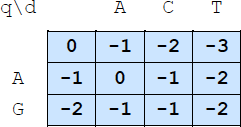
\includegraphics[width=0.3 \textwidth]{fig03/dp_distance_solution.png}
\end{figure}

%% (b)
  \part
   What is the edit distance between q and d?

  \begin{solution}[0.35 in]
  \begin{verbatim}
  2
  \end{verbatim}
  \end{solution}

  \vspace{0.1 in}

\end{parts}
